\subsection*{\underline{طراحی بخش DataBase}}

ما برای پروژه خود نیازمند دیتابیسی بودیم تا سوالات و پاسخ ها و یوزرهارا از آن فراخوانی کنیم.
برای این میتوانستیم از فایل استفاده کنیم یا با استفاده از $SQLite$ بر روی دیتابیس خود کوئری بزنیم.

اما تحقیق کردیم و دیدیم که یک لایبرری به نام Room وجود دارد که میتوان بدون نوشتن کوئری های SQL با دیتابیس کار کرد و کلاس های خود را به عنوان Entity در این دیتابیس تعریف کنیم.


	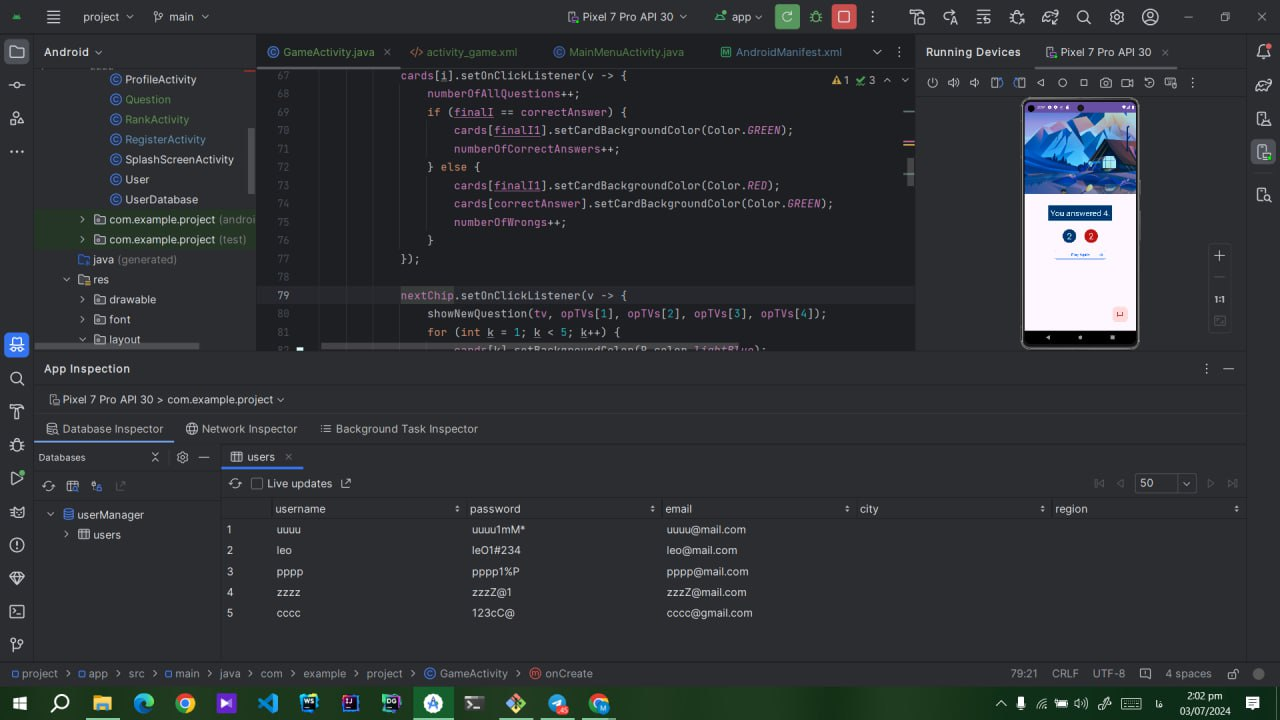
\includegraphics[width=1\linewidth]{screenshot004}

به عنوان مثال در عکس بالا، ما کلاس User را به عنوان یک Entity تعریف کردیم و Attribute های آن به عنوان ستون های دیتابیس ما در نظر گرفته می شوند.

